\documentclass[a4paper,12pt]{article} % добавить leqno в [] для нумерации слева
\usepackage[a4paper,top=1.3cm,bottom=2cm,left=1.5cm,right=1.5cm,marginparwidth=0.75cm]{geometry}
%%% Работа с русским языком
\usepackage{cmap}					% поиск в PDF
\usepackage[warn]{mathtext} 		% русские буквы в фомулах
\usepackage[T2A]{fontenc}			% кодировка
\usepackage[utf8]{inputenc}			% кодировка исходного текста
\usepackage[english,russian]{babel}	% локализация и переносы
\usepackage{physics}
\usepackage{multirow}

%%% Нормальное размещение таблиц (писать [H] в окружении таблицы)
\usepackage{float}
\restylefloat{table}

\usepackage{graphicx}

\usepackage{wrapfig}
\usepackage{tabularx}

\usepackage{hyperref}
\usepackage[rgb]{xcolor}
\hypersetup{
	colorlinks=true,urlcolor=blue
}

%%% Дополнительная работа с математикой
\usepackage{amsmath,amsfonts,amssymb,amsthm,mathtools} % AMS
\usepackage{icomma} % "Умная" запятая: $0,2$ --- число, $0, 2$ --- перечисление

%% Номера формул
%\mathtoolsset{showonlyrefs=true} % Показывать номера только у тех формул, на которые есть \eqref{} в тексте.

%% Шрифты
\usepackage{euscript}	 % Шрифт Евклид
\usepackage{mathrsfs} % Красивый матшрифт
\usepackage{pgfplots}
\pgfplotsset{compat=1.9}

%% Свои команды
\DeclareMathOperator{\sgn}{\mathop{sgn}}

%% Перенос знаков в формулах (по Львовскому)
\newcommand*{\hm}[1]{#1\nobreak\discretionary{}
	{\hbox{$\mathsurround=0pt #1$}}{}}

\date{\today}

\begin{document}

\begin{titlepage}
	\begin{center}
		{\large МОСКОВСКИЙ ФИЗИКО-ТЕХНИЧЕСКИЙ ИНСТИТУТ (НАЦИОНАЛЬНЫЙ ИССЛЕДОВАТЕЛЬСКИЙ УНИВЕРСИТЕТ)}
	\end{center}
	\begin{center}
		{\large Физтех-школа прикладной математики и информатики}
	\end{center}
	
	
	\vspace{4.5cm}
	{\huge
		\begin{center}
			{\bf Отчёт о выполнении лабораторной работы 4.3.1}\\
			
		\end{center}
	}
	\vspace{1cm}
	\begin{center}
		{\large Соболевский Федор Александрович \\
			\vspace{0.2cm}
			Б05-111}
	\end{center}
	\vspace{8cm}
	\begin{center}
		Март 2023
	\end{center}
\end{titlepage}

\section{Аннотация}
В данной работе на примере нескольких опытов исследовано явление дифракции. Проведены наблюдения и количественные измерения для разных видов дифракции - дифракции Френеля и дифракции Фраунгофера. Качественно и количественно проверены теоретические оценки для параметров дифракционных картин в каждом из опытов. На примере дифракции на двух щелях исследовано наложение друг на друга интерференционной и дифракционной картин. Выяснено, как дифракция влияет на разрешающую способность оптических инструментов.  

\section{Теоретические сведения}
Явление \textit{дифракции} суть явление отклонения в распространении света от законов геометрической оптики. В данной работе исследован частный случай дифракции: огибание световой волной малых препятствий.

Основными параметрами, определяющими вид дифракционной картины, являются расстояние до плоскости наблюдения $a$, длина волны $\lambda$ и характерный размер препятствия (например, ширина щели) $b$. При анализе видов дифракции используется \textit{волновой параметр} $p$, определяющийся как
\begin{equation} \label{waveParam}
    p = \frac{\sqrt{\lambda a}}{b}.
\end{equation}
В зависимости от значения $p$ дифракция называется \textbf{дифракцией Френеля} ($p \sim 1$) или \textbf{дифракцией Фраунгофера} ($p \gg 1$). При $p\ll 1$ явление дифракции практически не наблюдаемо, поэтому применимы приближения геометрической оптики.

\subsection*{Дифракция Френеля}
\begin{wrapfigure}{r}{0.45\textwidth}
  \begin{center}
    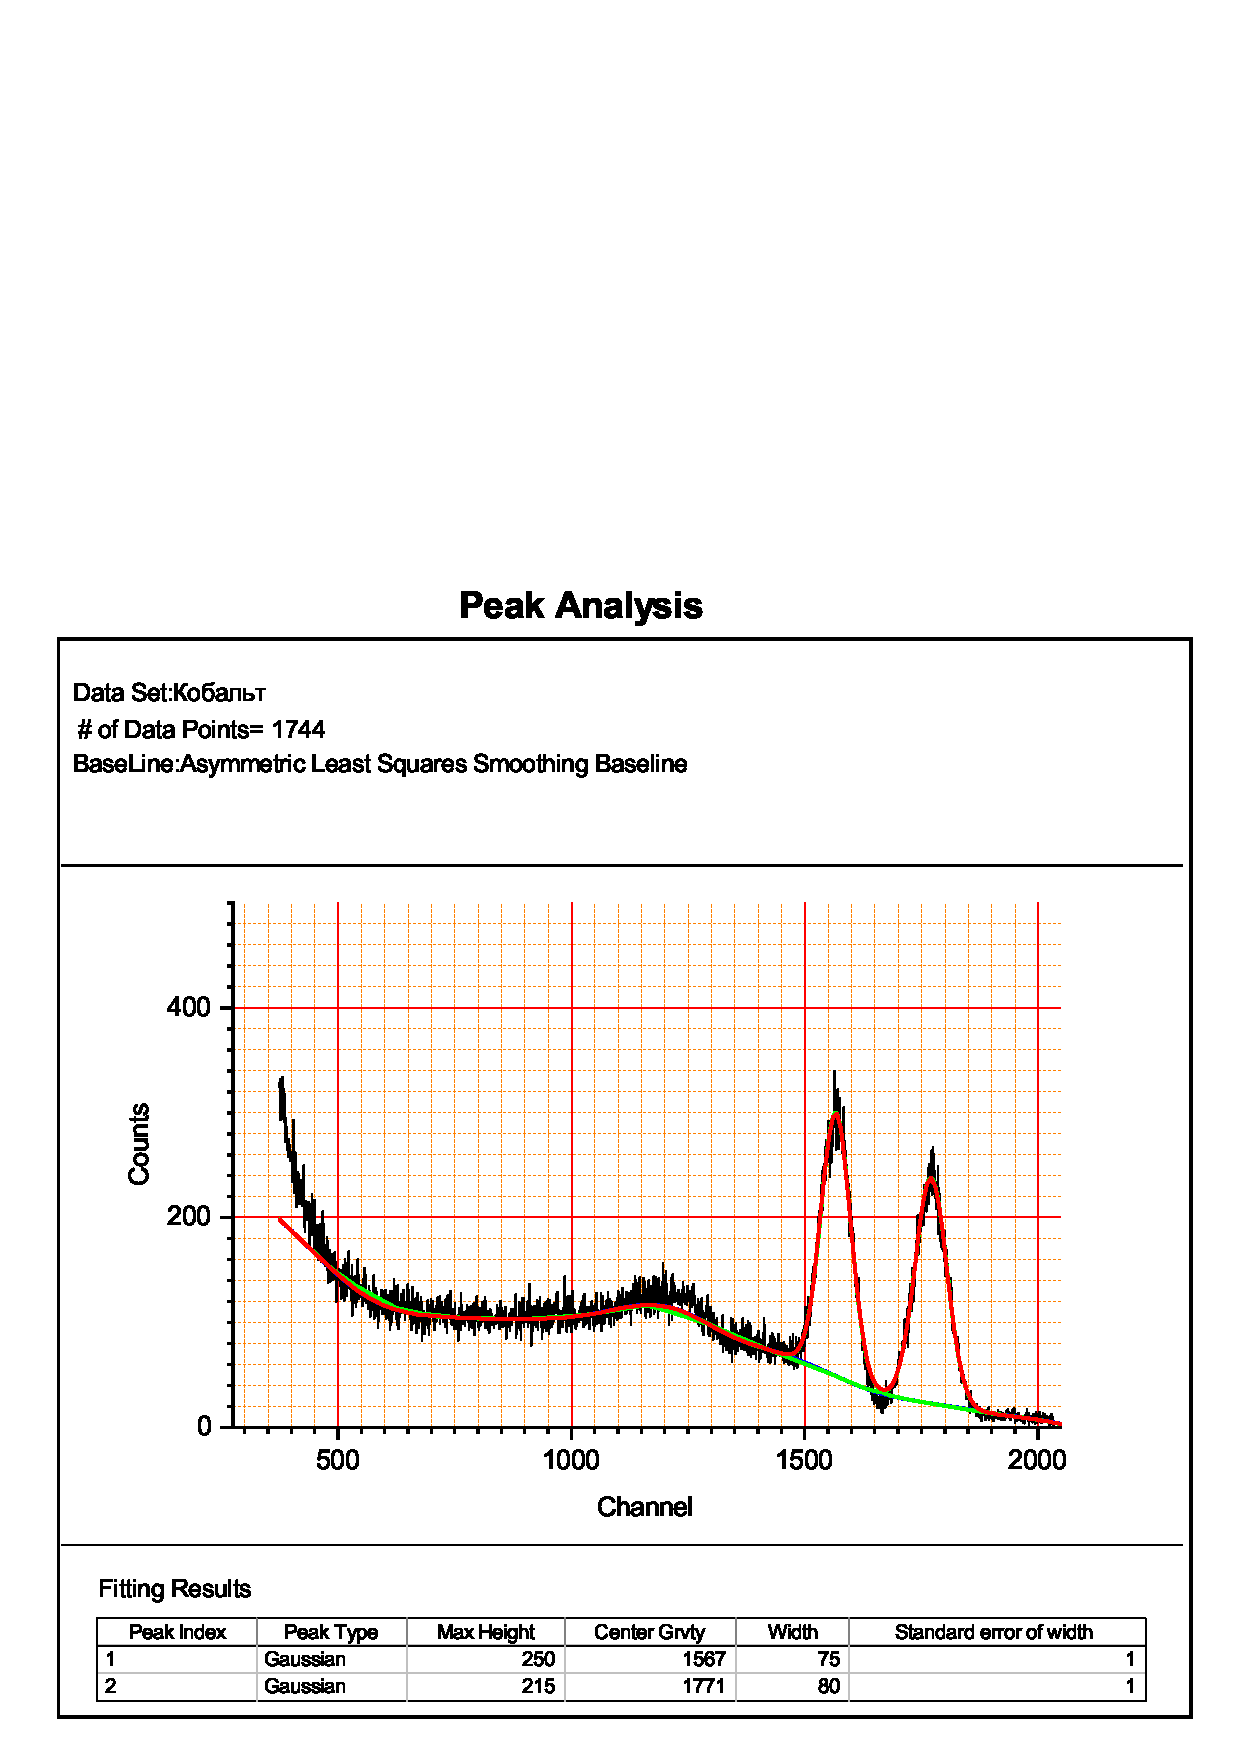
\includegraphics[width = 0.4\textwidth]{2.png}
  \end{center}
  \caption{Построение зон Френеля}
  \label{FrenellZones}
\end{wrapfigure}
Основной принцип, на котором основано явление дифракции~-- \textit{принцип Гюйгенса-Френеля}. Он формулируется следующим образом: \textit{Каждый элемент волнового фронта можно рассматривать как центр вторичного возмущения, порождающего вторичные сферические волны, а результирующее световое поле в каждой точке пространства будет определяться интерференцией этих волн.}

Данный принцип получил применение в \textit{зонной теории Френеля}. Рассмотрим действие световой волны действующей из точки $A$ в какой-то точке $B$ (см. рис. \ref{FrenellZones}). В этом случае можно, взяв точку $M_0$ в качестве центра, построить ряд концентрических сфер, радиусы которых начинаются с $b$ и увеличиваются каждый раз на половину длины волны $\lambda/2$. При пересечении с плоским фронтом волны $F$ эти сферы дадут концентрические окружности. Таким образом, на фронте волны появятся кольцевые зоны (зоны Френеля) с радиусами $r_1, r_2$ и т. д. Из геометрических соображений получаем радиус $m$-й зоны: 
\begin{equation}
r_m = m\sqrt{a\lambda}
\end{equation}
При $p\sim 1$ в ширину препятствия укладывается одна или несколько зон Френеля. При освещении тонкой щели параллельным пучком лучей (плоская зона) зоны Френеля прошедшего через щель света представляют собой плоскости, параллельные краям щели. Результирующая амплитуда в точке наблюдения определяется суперпозицией колебаний от тех зон Френеля, которые не перекрыты створками щели. Суммарная ширина $m$ зон Френеля $xi_m$ определяется соотношением
\begin{equation}
\xi_m = \sqrt{am\lambda},
\end{equation}
Вид наблюдаемой картины определяется \textit{числом Френеля} $\Phi$:
$$
\Phi^2 = \dfrac{b}{\sqrt{a\lambda}}
$$
-- число зон Френеля, которые укладываются в ширине щели $b$. Здесь волновой параметр $p = \frac{1}{\Phi^2}$.

\subsection*{Дифракция Фраунгофера}
\begin{wrapfigure}{r}{0.35\textwidth}
  \begin{center}
    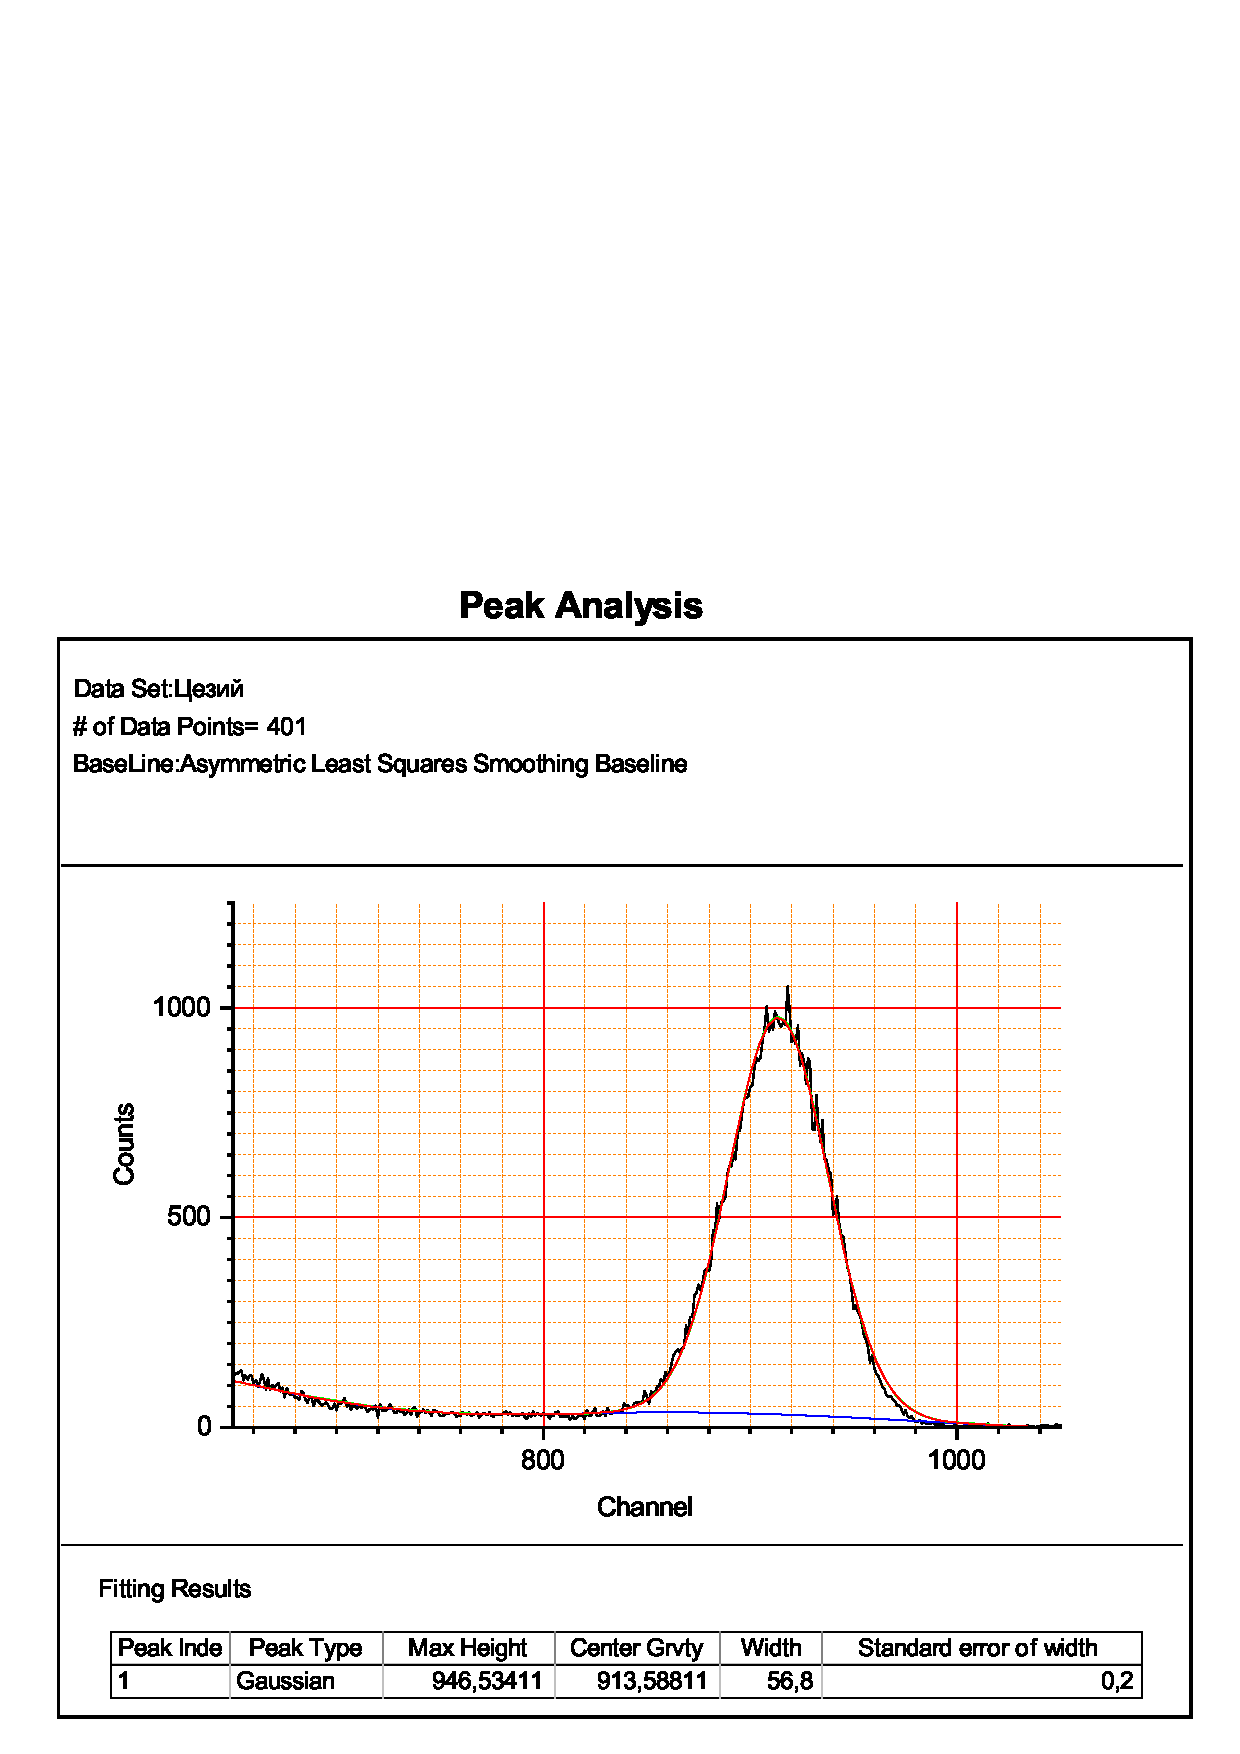
\includegraphics[width = 0.3\textwidth]{3.png}
  \end{center}
  \caption{К фазовым соотношениям при дифракции Фраунгофера}
  \label{FHDiff}
\end{wrapfigure}
В этом пункте рассмотрим дифракцию, когда ширина щели становится значительно меньше ширины первой зоны Френеля, т.е. если 
\begin{equation}
    b \ll\sqrt{a \lambda} 
\end{equation}	
Это условие всегда выполняется при достаточно большом $a$. Схематично ход лучей при дифракции Фраунгофера изображён на рис. \ref{FHDiff}. Разность хода между соседними лучами определяется как 
\begin{equation}
\Delta = r_2 - r_1 \approx D \sin \theta \approx D \cdot \theta
\end{equation}
в предположении, что $\theta$ достаточно мал.

Для дифракции Фраунгофера на щели справедливы следующие выражения для угловой координаты $m$-й темной полосы:
\begin{equation}
\theta_m = \frac{m \lambda}{b};
\end{equation}
и расстояния до неё от центра: 
\begin{equation}
X_m = m\frac{\lambda}{b}.
\end{equation}

В случае, когда вместо одной щели две на расстоянии $d$ друг от друга, на дифракционную картину накладывается также интерференционная. Ширина интерференционной полосы определяется как
\begin{equation}
    \delta x = a\frac{\lambda}{d}.
\end{equation}
Число интерференционных полос, укладывающихся в области центрального максимума, в этом случае равно
\begin{equation}
n = \frac{2d}{b}
\end{equation}

\subsection*{Влияние дифракции на разрешающую способность оптического инструмента}
Из-за дифракции изображения точек, расположенных на близком расстоянии друг к другу, могут сливаться, что влияет на разрешающую способность оптических систем, в которых присутствуют малые щели. Величина оптического искажения зависит от углового расстояния между объектами относительно оптической системы:
\begin{equation}
\varphi = \frac{d}{f_1},
\end{equation}
где $f_1$~-- расстояние от объекта до системы. В данной работе искажения вследствие дифракции наблюдались для изображений двух тонких щелей на расстоянии $d$ друг от друга. Расстояние $l$ между изображениями щелей равно 
\begin{equation}
l = \varphi \cdot a = d\frac{a}{f_1}, 
\end{equation}
а ширина изображений вследствие дифракции
\begin{equation}
    \delta x \approx \frac{\lambda}{b}a.
\end{equation}
Изображения двух щелей различимы, если полуширина дифракционных полос меньше расстояния между изображениями, т.\,е. минимальное допустимое расстояние между различимыми точками определяется из соотношения
\begin{equation}
\delta x \sim l \Rightarrow \frac{\lambda}{b} \sim \frac{d}{f_1}.
\end{equation}

\section{Ход работы}

\subsection*{А. Дифракция Френеля на одной щели}
\begin{figure}[h]
    \centering
    \includegraphics[width=0.7\textwidth]{frenelSetup.png}
    \caption{Схема установки для наблюдения дифракции Френеля}
    \label{fig:frenel}
\end{figure}

Схема экспериментальной установки изображена на рис. \ref{fig:frenel}. Свет из монохроматора преобразуется в параллельный пучок и направляется на щель $S_2$ достаточно большой (относительно параметра $p$) ширины $b$. Дифракционная картина в плоскости П наблюдается с помощью микроскопа М. 

С помощью микрометрического винта измерим ширину щели: $ b = 0,16 \pm 0,02 $ мм. Приближая микроскоп к щели, снимем зависимость координаты микроскопа $a_n$ от числа $ n $ темных полос по формуле $ a_n = x_n - x_0 $, где $ x_0 = 58,4 $ мм~-- положение нуля. Результаты измерений и вычисления $2\xi_m$ представлены в таблице \ref{tab:frenel}. Длина волны зеленой линии света ртутной лампы равна $ \lambda = 546,1 \cdot 10^{-6} $ мм.
\begin{table}[h!]
\caption{Зависимость координаты микроскопа от числа $ n $ темных полос}
\begin{center}
	\begin{tabular}{|c|c|c|c|c|}
		\hline
		$ x_n $, мм & $ n $ & $ a_n $, мм & $ 2\xi_n $, мкм &                    $\sigma_{\ksi}$, мкм \\
		\hline
		  574 & 6 & 10 & 181 & 11 \\
		573 & 4 & 11 & 155 & 9\\
		570 & 3 & 14 & 151 & 9 \\
            567 & 2 & 17 & 136 & 7\\
            558 & 1 & 26 & 119 & 6\\
		\hline
	\end{tabular}
\end{center}
\label{tab:frenel}
\end{table}

Усредняя, получаем экспериментальное значение ширины щели: $b = 149 \pm 14$ мкм. Это значение совпадает с измеренной микрометрическим винтом величиной $b$ в пределах погрешности измерений.

\subsection*{Б. Дифракция Фраунгофера на одной щели}
\begin{figure}[h]
    \centering
    \includegraphics{fraunhoferSetup.png}
    \caption{Схема установки для наблюдения дифракции Фраунгофера на одной щели}
    \label{fig:FH1hole}
\end{figure}

Схема экспериментальной установки для исследования дифракции Фраунгофера на одной щели изображена на рис. \ref{fig:FH1hole}. Соотношение параметров $a$, $b$ и $\lambda$ теперь удовлетворяет условию $p\gg 1$, а изображение дифракционной картины дополнительно увеличивается линзой $O_2$.

Измеренная с помощью микрометрического винта ширина щели равна $ b =  0,28 \pm 0,01 $ мм. Фокусное расстояние линзы $ f_2 = 11 $ см. Измерим с помощью винта поперечного перемещения микроскопа координаты $ X_m $ нескольких дифракционных минимумов. Здесь $ x_m $~-- измерения, которые затем умножаем на $ \alpha = 0,02 $ мм~-- цену деления винта, т.е. $ X_m = \alpha x_m $.
 Результаты представлены в таблице \ref{tab:tab} и на графике \ref{A}. 
 
\begin{table}[]
    \centering
		\begin{tabular}{|c|c|c|}
			\hline
			$ x_m $ & $ X_m $, мм & $ m $ \\
			\hline
                -64 & -1.28 & -5\\
			-47 & -0.94 & -4\\
			-39 & -0.78 & -3\\
			-23 & -0.46 & -2\\
			-13 & -0.26 & -1\\
			14 & 0.28 & 1\\
			24 & 0.48 & 2\\
			37 & 0.74 & 3\\
			49 & 0.98 & 4\\ 
                62 & 1.24 & 5\\
			\hline
		\end{tabular}
  \label{tab:tab}
\end{table}

\begin{figure}[h!]
    \centering
    \includegraphics[width = 0.8\textwidth]{B.jpg}
    \caption{График зависимости суммарной ширины зон Френеля от их числа}
    \label{A}
\end{figure}

Из аппроксимации экспериментальных данных следуеет, что расстояние между соседними максимумами $ a = 0,247 \pm 0,007$ мм. Из теоретических оценок получаем, что 
\begin{equation}\label{}
b = \x \dfrac{\lambda}{a} f_2 = 0,241 \pm 0,010 \; \text{мм}. 
\end{equation}
Это значение совпадает с полученным экспериментальным путём в пределах погрешности измерений.

\subsection*{В. Дифракция Фраунгофера на двух щелях}
\begin{figure}
    \centering
    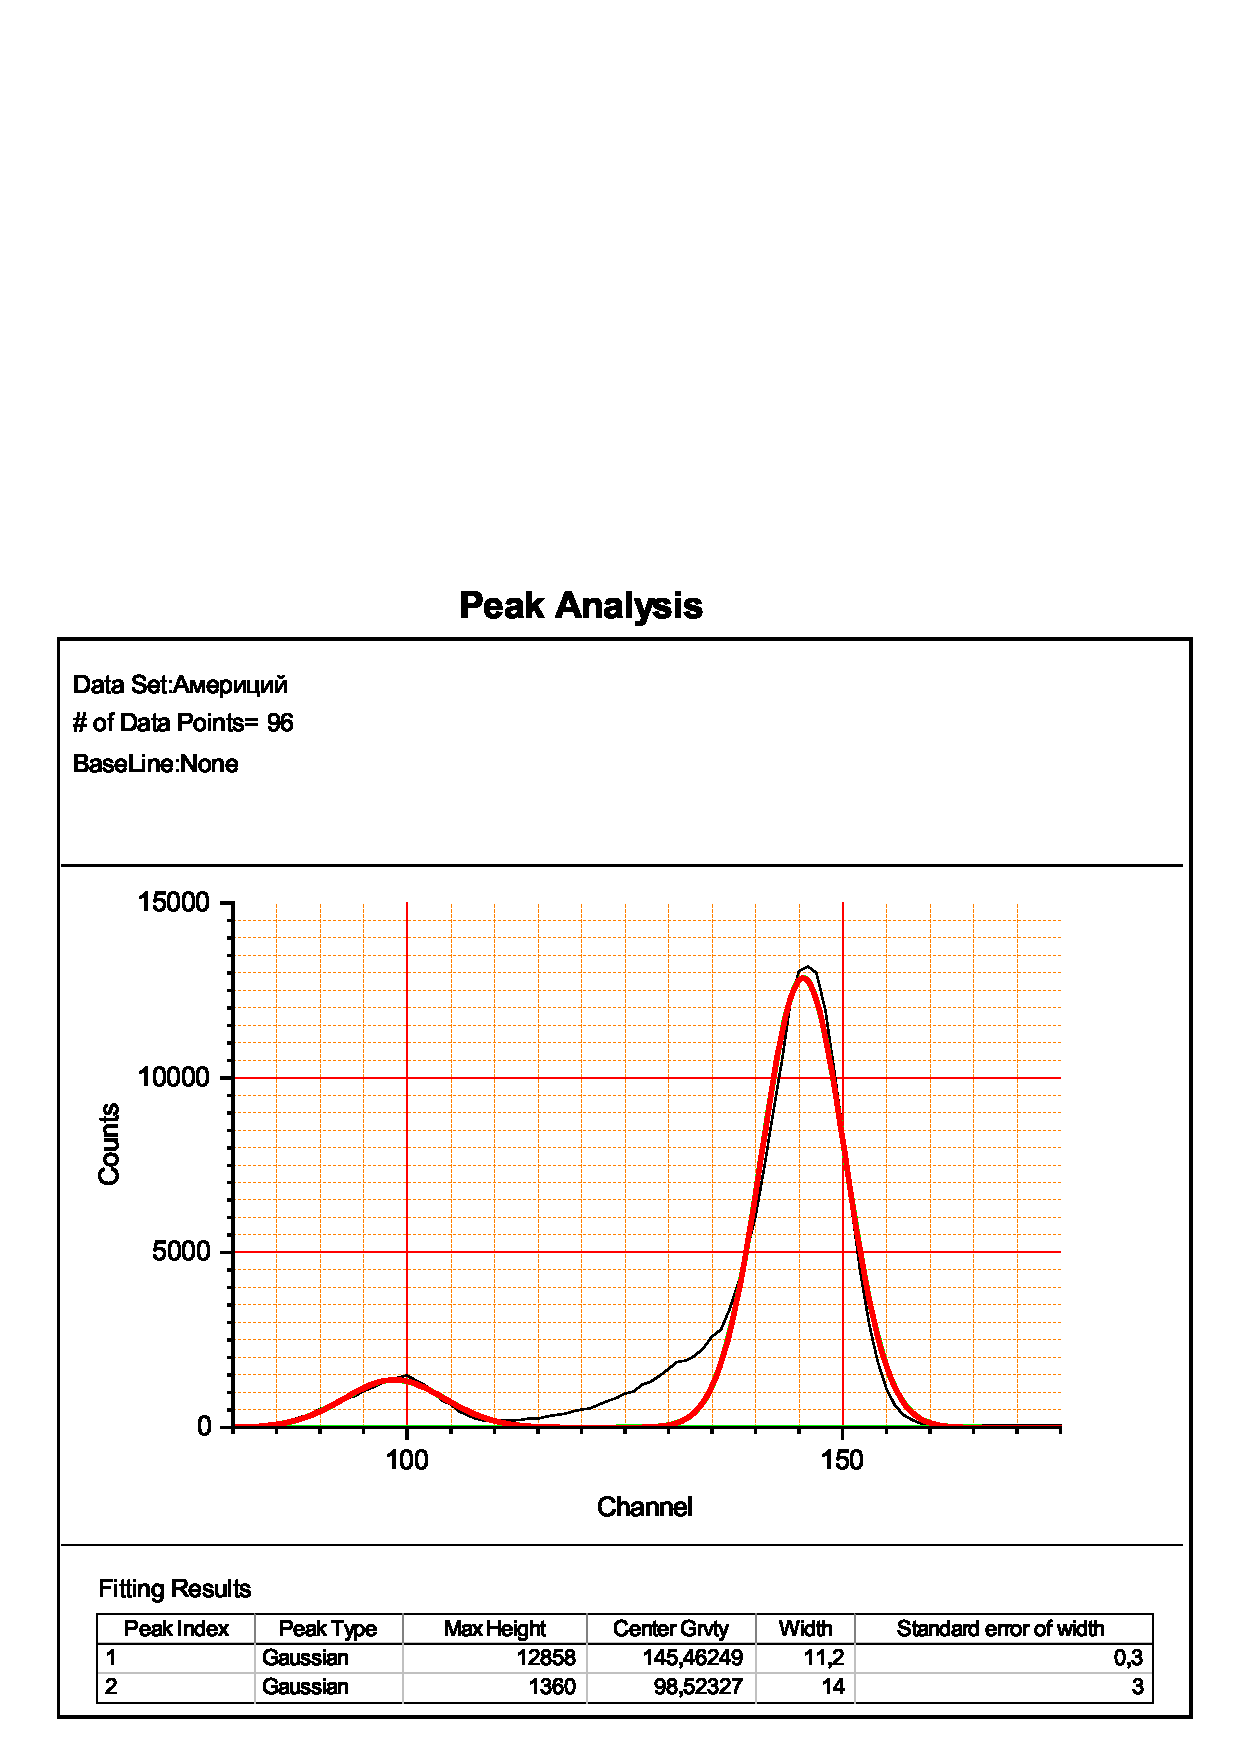
\includegraphics{5.png}
    \caption{Схема установки для наблюдения дифракции Фраунгофера на двух щелях}
    \label{fig:FH2holes}
\end{figure}
Схема экспериментальной установки для исследования дифракции Фраунгофера на двух щелях изображена на рис. \ref{fig:FH2holes}. В данном опыте на полученную дифракционную картину накладывается также интерференционная. Расстояние между крайними минимумами $l = 0,34 \pm 0,01$ мм. В главном максимуме наблюдаем $n = 12$ светлых полос, поэтому
\begin{equation}
    \delta x = \frac{l}{n} = 28.3 \pm 0.8 \; \text{мкм}
\end{equation}
Расстояние между щелями и ширина щели равны соответственно
 \begin{equation}
 d = f_2 \dfrac{\lambda}{\delta x} = 2,31 \pm 0,07 \; \text{мм}
 \end{equation}

  \begin{equation}
 b = 0,36 \pm 0,01 \; \text{мм}
 \end{equation}
 
 Отсюда находим $n_{th}$~-- теоретическое количество светлых полос в главном максимуме
   \begin{equation}\label{}
n = \frac{2d}{b} = 12,9 \pm 0,6
 \end{equation}
 Это значение совпадает с наблюдаемым в пределах двух стандартных отклонений. Первое исчезновение интерференционных полос при $b_0 = 27 \pm 1$ мкм. Теоретическая оценка: 
 \begin{equation}\label{}
 b_{th} = \dfrac{f_1 \lambda}{d} = 23,3 \pm 0,6\; мм
 \end{equation}
 Здесь отклонение уже сущетственно больше погрешности измерений и составляет около 14\%. 
 
\subsection*{Г. Влияние дифракции на разрешающую способность оптической системы}
\begin{figure}
    \centering
    \includegraphics{6.png}
    \caption{Схема установки для наблюдения ухудшения качества изображений из-за дифракции}
    \label{fig:bad}
\end{figure}

Схема экспериментальной установки для исследования влияния дифракции на разрешающую способность оптической системы изображена на рис. \ref{fig:bad}.
Поставив между линзами щель $S_2$ и уменьшая ее ширину, визуально фиксируем ухудшение изображения. Подбираем ширину $S_2$ так, чтобы изображения почти сливались.
\[b_0 = 0,03\text{ мм}\]
Расстояние между щелями $d = 1,70 \text{мм}$. Воспользовавшись критерием Рэлея, найдем
\begin{equation}
    b_0^{theor} = f_1 \frac{\lambda}{d} = 35,3 \pm 0,3\; \text{мкм}.
\end{equation}

Экспериментальное и теоретическое значения равны в пределах двух стандартных отклонений. Главное, что требовалось пронаблюдать~-- то, что эти значения совпадают по порядку величины, т.\,е. действительно верен критерий Релея.

\section{Выводы}

В ходе выполнения лабораторной работы удалось пронаблюдать основные виды дифракции: дифракцию Френеля и дифракцию Фраунгофера. Полученные с помощью теоретических расчётов значения ширины щели в пределах погрешности измерений совпали с измеренными инструментально. Это позволяет говорить о том, что приведённые соотношения для дифракции применимы для данного опыта, поскольку приближения, использованные при их выводе, дают ошибку измерений не больше инструментальной.

В ходе опыта на дифракцию на двух щелях удалось получить одновременно дифракционную и интерференционную картины. При этом полученная картина соответствует теоретическому ожиданию. Это подтверждает тот факт, что дифракция Фраунгофера и двухщелевая интерференция имеют одинаковую природу, но зависят от разных параметров.

Кроме того, мы опытным путём установили, что дифракция ограничивает разрешающую способность оптического инструмента, что приводит к снижению качества изображения. При этом критерий Рэлея оказался выполнен, что говорит о его применимости для оценки разрешающей способности оптических систем.


\end{document}